\documentclass[11pt,a4paper]{article}

% ------------------------------------------------------------------
% Packages
% ------------------------------------------------------------------
\usepackage[utf8]{inputenc}
\usepackage[T1]{fontenc}
\usepackage{lmodern}
\usepackage[english]{babel}
\usepackage{amsmath, amssymb, amsthm, mathtools}
\usepackage[margin=2.4cm]{geometry}
\usepackage{hyperref}
\usepackage{graphicx}
\graphicspath{{../scripts/figures/}}
\usepackage{xcolor}
\usepackage{booktabs}
\usepackage{enumitem}
\usepackage{siunitx}
\usepackage{bm}
\usepackage{authblk}
\usepackage{tikz}
\usetikzlibrary{arrows.meta, positioning}

\hypersetup{
  colorlinks=true,
  linkcolor=blue!60!black,
  citecolor=blue!60!black,
  urlcolor=blue!60!black
}

\theoremstyle{plain}
\newtheorem{proposition}{Proposition}

\newcommand{\dv}{\Delta v}

\title{\textbf{High-Fidelity Closed-Loop Low-Thrust Trajectory Design\\
with a Quantum-Ready Binary Scheduler}\\[2pt]
\large GMAT-in-the-loop QUBO optimization and a SMART-1 case study}

\author[1]{Gino Luciano Moretta\thanks{morettaginoluciano@gmail.com}}
\author[1]{Antonio Paolozzi}
\affil[1]{School of Aerospace Engineering, Sapienza Universit\`a di Roma}

\date{June 2026 --- working note (v3)}

\begin{document}
\maketitle

% ------------------------------------------------------------------
\begin{abstract}
% ------------------------------------------------------------------
We extend our binary-schedule QUBO transcription of low-thrust trajectory
design from an in-house planar circular restricted three-body (CR3BP)
propagator to a \emph{high-fidelity closed loop} in which NASA's General
Mission Analysis Tool (GMAT) plays the role of the truth model. A Python
layer orchestrates the loop: it writes GMAT mission scripts, runs them
headless, measures each candidate burn's effect on the spacecraft state by
finite differences \emph{within the real dynamics}, assembles a quadratic
unconstrained binary optimization (QUBO) over the engine's on/off schedule,
solves it, and validates the chosen schedule back in GMAT under a
trust-region accept rule. The QUBO is solved classically here, but it is the
exact form a quantum annealer ingests, so the combinatorial step is
hardware-swappable with no change to the formulation. We exercise the loop on
ESA's SMART-1 electric-propulsion transfer, starting from its published
geostationary transfer orbit (GTO) and Hall thruster: the orbit-raising
budget matches the flown mission, the optimizer rediscovers the Oberth
perigee-thrust strategy on its own under a duty-cycle constraint, and a
launch-epoch phase search produces a real lunar encounter that the binary
scheduler brakes into a bound lunar orbit. We characterise the computational
profile (dominated by high-fidelity propagation, linear in the number of
decision slots, not exponential), explain why the loop never simulates the
$2^{N}$ burn combinations, and close with an applied outlook: autonomous
on-board maneuver planning and a concrete path to quantum hardware for large,
dense scheduling problems.
\end{abstract}

\noindent\textbf{Keywords:} low-thrust trajectory optimization, QUBO, quantum
annealing, GMAT, sequential linearization, trust region, lunar capture,
SMART-1, autonomous guidance.

% ==================================================================
\section{Introduction and relation to the previous work}
% ==================================================================
A companion note (v2) posed low-thrust cislunar trajectory correction as a
\emph{naturally binary} QUBO: at each of $N$ time steps an on/off command
$q_i\in\{0,1\}$ decides whether a constant-thrust engine fires, and the
schedule that best reaches a target is the ground state of a QUBO assembled
from a first-order state-transition-matrix expansion. That work was developed
and validated entirely in an \emph{in-house} planar CR3BP propagator: a fast,
transparent model, ideal for deriving the method and proving its
monotonicity, but an idealised one (planar, nondimensional, three point
masses, fixed-step RK4).

The natural and most frequent objection to any such result is: \emph{would the
schedule survive real dynamics?} This note answers it by replacing the
in-house propagator with NASA GMAT~\cite{GMAT} as the truth model --- full
DE-series ephemerides, Earth gravity field, Moon and Sun, finite burns, mass
depletion --- while keeping the same binary-QUBO decision layer. The result is
a closed \emph{design$\rightarrow$simulate$\rightarrow$read$\rightarrow$decide}
loop, the automated analogue of the write--run--read--fix cycle an engineer
uses, with a high-fidelity simulator in the loop rather than a toy model.

The contributions of this note are:
\begin{enumerate}[leftmargin=1.5em, itemsep=2pt]
  \item A high-fidelity closed-loop architecture (Sec.~\ref{sec:method}) in
    which Python orchestrates GMAT and a QUBO solver, with the
    impulse-response sensitivities measured by finite differences in the
    truth model itself.
  \item A clear account (Sec.~\ref{sec:no2N}) of why the loop is tractable ---
    why it never simulates the $2^{N}$ burn combinations --- which is the
    crux of any linearization-based optimizer.
  \item A SMART-1 case study (Sec.~\ref{sec:smart1}) from the real launch
    orbit: orbit-raising budget, a self-discovered Oberth strategy, a real
    lunar encounter, and a binary-scheduled capture, with honest limits.
  \item A computational and quantum-readiness analysis (Sec.~\ref{sec:cost})
    and an applied outlook (Sec.~\ref{sec:outlook}) on on-board autonomy and
    quantum hardware.
\end{enumerate}

% ==================================================================
\section{Method: a high-fidelity closed loop}\label{sec:method}
% ==================================================================
Three components, with disjoint roles, exchange data in a loop
(Fig.~\ref{fig:loop}).

\paragraph{GMAT --- the truth.} GMAT never optimizes. It answers one question
exactly: \emph{given this on/off firing pattern, what is the resulting state?}
We script a spacecraft with an electric thruster and a force model (Earth
$4\times4$ gravity, Moon and Sun as point masses, DE405 ephemerides), run it
headless via a subprocess, and parse the report file.

\paragraph{Python --- the orchestrator and the brain.} Python templates the
GMAT scripts, launches the runs (in parallel), reads the results, assembles
the QUBO, solves it, and applies the accept/reject logic.

\paragraph{The QUBO --- the combinatorial decision.} A quadratic binary
objective whose minimiser is the firing pattern. It is solved here by exact
enumeration (for $N\!\le\!20$) or simulated annealing, but it is written in
the canonical form
$\min_{\bm q\in\{0,1\}^N}\ \bm q^\top \bm Q\,\bm q + \bm\ell^\top\bm q$
that a quantum annealer accepts natively.

\begin{figure}[t]
\centering
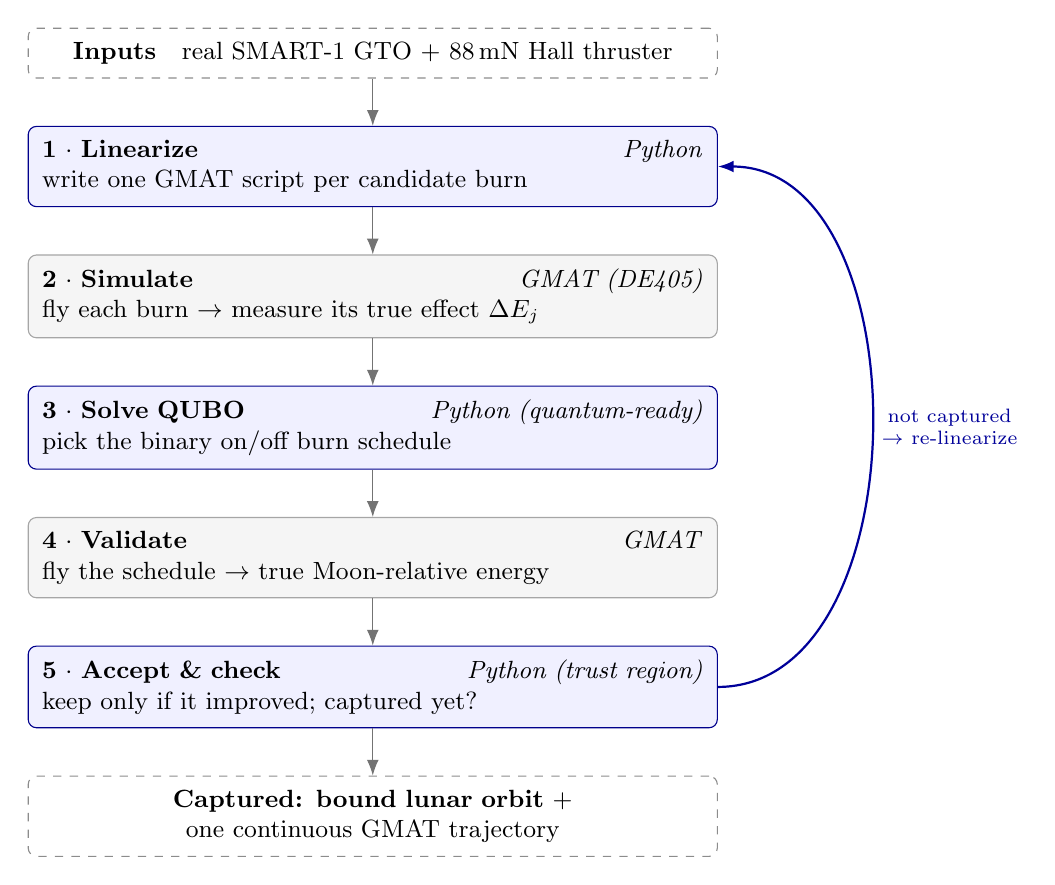
\begin{tikzpicture}[
  node distance=6mm and 0mm,
  box/.style={rounded corners=3pt, draw, align=left, text width=8.4cm,
              inner sep=5pt, font=\small},
  py/.style={box, fill=blue!6, draw=blue!55!black},
  gm/.style={box, fill=black!4, draw=black!35},
  io/.style={box, dashed, draw=black!45, fill=none, align=center},
  fl/.style={-{Latex[length=2mm]}, draw=black!55},
  lp/.style={-{Latex[length=2mm]}, draw=blue!60!black, thick}
]
\node[io] (in) {\textbf{Inputs}\quad real SMART-1 GTO $+$ \SI{88}{\milli\newton} Hall thruster};
\node[py, below=of in] (p1) {\textbf{1 $\cdot$ Linearize} \hfill \textit{Python}\\ write one GMAT script per candidate burn};
\node[gm, below=of p1] (g1) {\textbf{2 $\cdot$ Simulate} \hfill \textit{GMAT (DE405)}\\ fly each burn $\to$ measure its true effect $\Delta E_j$};
\node[py, below=of g1] (p2) {\textbf{3 $\cdot$ Solve QUBO} \hfill \textit{Python (quantum-ready)}\\ pick the binary on/off burn schedule};
\node[gm, below=of p2] (g2) {\textbf{4 $\cdot$ Validate} \hfill \textit{GMAT}\\ fly the schedule $\to$ true Moon-relative energy};
\node[py, below=of g2] (p3) {\textbf{5 $\cdot$ Accept \& check} \hfill \textit{Python (trust region)}\\ keep only if it improved; captured yet?};
\node[io, below=of p3] (out) {\textbf{Captured: bound lunar orbit} $+$ one continuous GMAT trajectory};

\draw[fl] (in) -- (p1);
\draw[fl] (p1) -- (g1);
\draw[fl] (g1) -- (p2);
\draw[fl] (p2) -- (g2);
\draw[fl] (g2) -- (p3);
\draw[fl] (p3) -- (out);
\draw[lp] (p3.east) .. controls +(2.6,0) and +(2.6,0) .. node[right, font=\scriptsize, text=blue!60!black, align=center]{not captured\\$\to$ re-linearize} (p1.east);
\end{tikzpicture}
\caption{The closed loop. Blue $=$ Python (orchestrator $+$ QUBO optimizer);
grey $=$ GMAT (high-fidelity simulator, the ``truth''). Steps 1--2 build a
model from real physics; step 3 makes the combinatorial decision; steps 4--5
validate it and decide whether to repeat. Phase 1 (the GTO$\to$Moon spiral)
uses the same write--run--read loop with continuous thrust.}
\label{fig:loop}
\end{figure}

\subsection{The binary scheduling QUBO}
Over one maneuver window of duration $T$ split into $N$ equal slots, let
$\Delta E_j$ be the change in a scalar objective (here the Moon-relative
specific energy, or more generally a weighted final-state miss) produced by
firing \emph{only} slot $j$, measured in GMAT. The first-order model assumes
the slot effects superpose,
\begin{equation}\label{eq:lin}
  E(\bm q)\ \approx\ E_0 + \sum_{j=1}^{N} q_j\,\Delta E_j ,
\end{equation}
and the schedule that drives $E$ to a target $E_\star$ with the fewest burns
is the minimiser of
\begin{equation}\label{eq:qubo}
  f(\bm q)\ =\ \Big(\textstyle\sum_j q_j\,\Delta E_j - d\Big)^2
              + \alpha \sum_j q_j ,
  \qquad d = E_\star - E_0 ,
\end{equation}
which expands to $\bm q^\top\bm Q\,\bm q + \bm\ell^\top\bm q + \text{const}$
with $\bm Q = \Delta\bm E\,\Delta\bm E^\top$ and
$\bm\ell = \alpha\bm 1 - 2d\,\Delta\bm E$. The fuel weight $\alpha$ is a small
tiebreaker; the energy term must dominate it, or the optimizer refuses to
brake.

\subsection{The outer loop: sequential re-linearization with a trust region}
Equation~\eqref{eq:lin} is only first-order. After the QUBO returns a
candidate $\hat{\bm q}$, we fly the \emph{actual} schedule in GMAT and read the
true energy. The candidate is accepted only if the true miss improved; the
loop then re-linearises around the new schedule and repeats, terminating at a
fixed point or when no candidate improves. This is the binary analogue of
sequential convex programming with a trust-region safeguard, and it is
monotone: it can never return a schedule worse than coasting. For the
near-parabolic SMART-1 capture a single window suffices; long arcs are handled
by chaining short windows (a receding-horizon / model-predictive structure).

% ==================================================================
\section{Why the loop never simulates $2^{N}$ combinations}\label{sec:no2N}
% ==================================================================
It is tempting to think that choosing among $2^{N}$ firing patterns requires
simulating them. It does not, and this is the heart of the method.

We measure each burn's effect \emph{individually} --- $N$ single-slot GMAT
runs --- and the QUBO \emph{assumes the effects add} (Eq.~\ref{eq:lin}). The
true dynamics couple the burns (firing slot $A$ shifts the state, so slot $B$
acts slightly differently), and that coupling is \emph{not} measured; it is the
modelling error. The safeguard is the outer loop: we fly the one chosen
combination in GMAT (step 4) and verify it; if superposition was too
optimistic, the trust-region rule rejects the step or we re-linearise. Hence
\begin{center}
\emph{$N$ runs to build the model $+$ 1 run to validate the chosen
combination, per iteration --- never $2^{N}$.}
\end{center}
The exponential search lives entirely in the \emph{cheap} QUBO: evaluating the
quadratic form $2^{N}$ times costs microseconds, not GMAT propagations. The
expensive, high-fidelity simulator is touched only $N{+}1$ times per pass plus
one validation. This is the classic bargain of linearization-based
optimization --- measure the pieces, assume they compose, verify the answer ---
and the trust region is what makes ``assume they compose'' safe.

% ==================================================================
\section{Case study: re-flying SMART-1 from its real GTO}\label{sec:smart1}
% ==================================================================
ESA's SMART-1 reached the Moon by spiralling out of a geostationary transfer
orbit with a single PPS-1350 Hall thruster over $\sim$14
months~\cite{Racca2002,Milligan2005}. We take its published inputs: GTO
$654\times\SI{35885}{\km}$ altitude, $i=\ang{7}$; Hall thruster
\SI{88}{\milli\newton}, $I_{sp}=\SI{1650}{\second}$; wet mass \SI{367}{\kg},
\SI{82}{\kg} xenon. Everything below runs in GMAT R2025a under real
ephemerides (Earth $4\times4$, Moon, Sun).

\subsection{Phase 1 --- the orbit-raising spiral}
Continuous tangential thrust raises the apogee from GTO to lunar distance in
\SI{140}{\day} at 100\,\% duty, costing $\dv\approx\SI{3180}{\meter\per\second}$
and \SI{65.8}{\kg} of xenon, with the inclination essentially held
($\ang{7.0}\!\to\!\ang{6.42}$). SMART-1 flew
$\approx\SI{3500}{\meter\per\second}$ over $\sim\SI{410}{\day}$ (including
capture) at $\sim40\,\%$ duty; at that duty our \SI{140}{\day} becomes
$\sim\SI{350}{\day}$. The agreement is the physics check: the orbit-raising
$\dv$ is the (thrust-independent) Edelbaum invariant
(Fig.~\ref{fig:spiral})~\cite{Edelbaum1961}.

\begin{figure}[t]
\centering
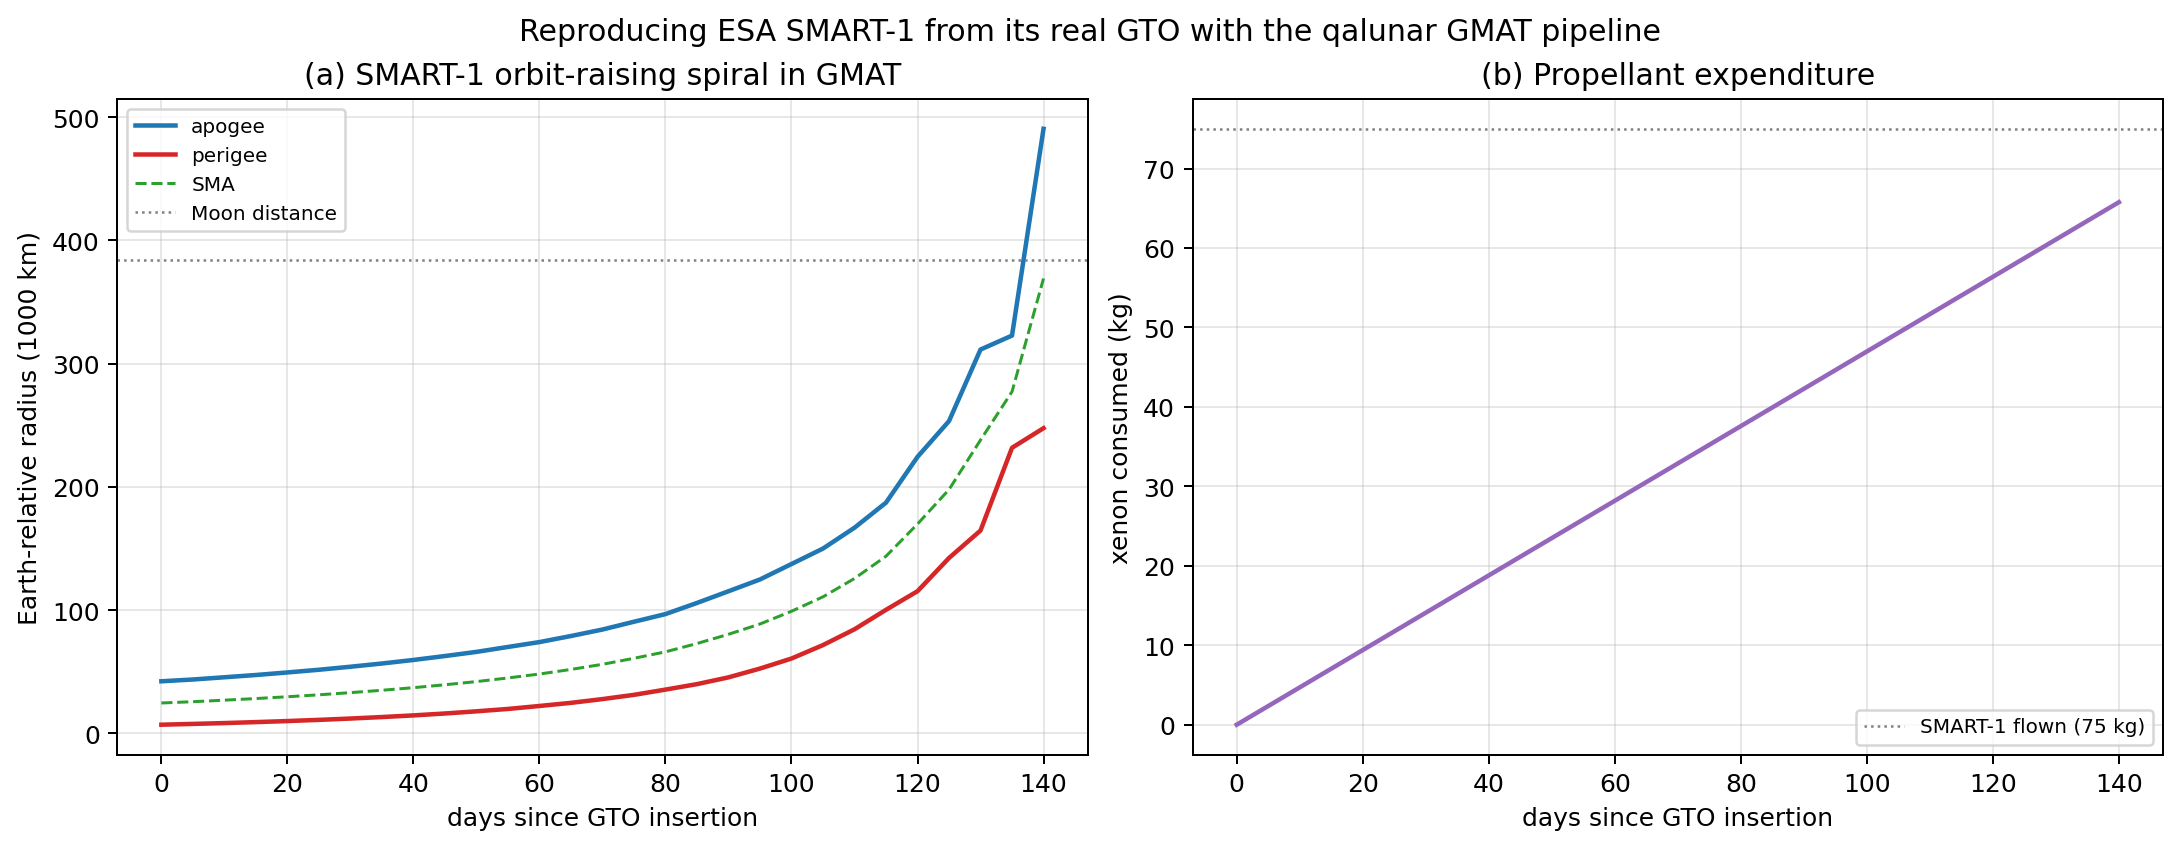
\includegraphics[width=\textwidth]{smart1_gmat_spiral.png}
\caption{SMART-1 orbit-raising spiral reproduced in GMAT from the real GTO.
\emph{Left:} apogee/perigee/SMA climbing toward lunar distance. \emph{Right:}
xenon expended (linear), with the flown total marked.}
\label{fig:spiral}
\end{figure}

\subsection{The optimizer rediscovers the Oberth effect}
SMART-1 could fire only $\sim40\,\%$ of each orbit (power, eclipse, thermal
limits), so the operative question is \emph{which arc} to thrust. We split one
GTO orbit into $N=24$ time slots, measure each slot's energy gain
$\Delta E_j$ in GMAT, and pose ``raise energy with a budget of
$K=\lfloor0.4N\rfloor=10$ burns'' as a QUBO. The measured $\Delta E_j$ is
linear in the slot speed --- the Oberth law $\mathrm dE=v\,\mathrm dv$, recovered
empirically --- and the optimizer, with no orbital-mechanics knowledge,
clusters all ten burns at perigee (Fig.~\ref{fig:oberth}). Validated in GMAT,
the perigee schedule raises apogee \SI{120}{\km} per orbit against \SI{64}{\km}
for evenly-spread firing ($1.9\times$) and \SI{9.8}{\km} for apogee-clustered
firing --- the same maximum-efficiency strategy SMART-1 flew operationally,
derived here from the discrete side. (The dense, all-to-all cardinality QUBO
is, notably, hard enough that classical simulated annealing did not reach its
exact ground state at $N=24$, motivating exact or quantum solvers.)

\begin{figure}[t]
\centering
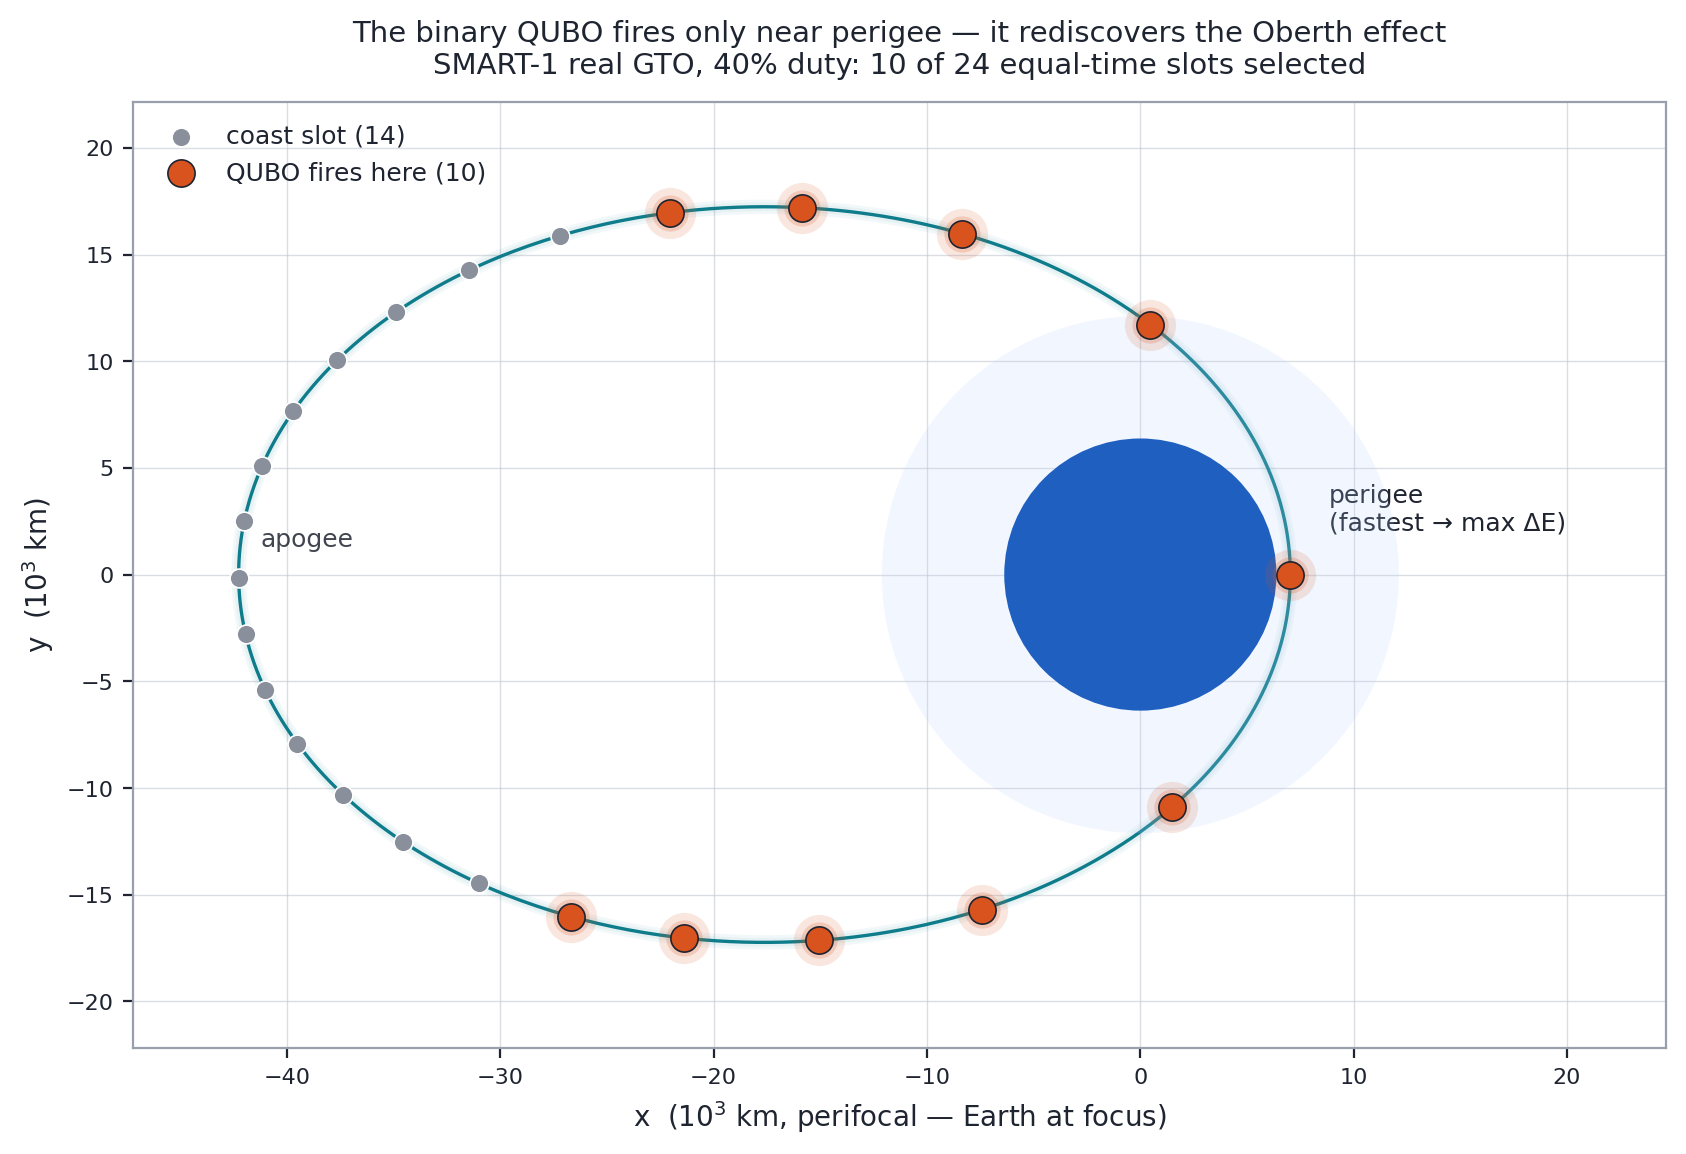
\includegraphics[width=\textwidth]{smart1_duty_cycle.png}
\caption{Under a 40\,\% duty constraint the binary optimizer rediscovers
Oberth. \emph{(a)} measured energy gain per burn is linear in slot speed
($\mathrm dE=v\,\mathrm dv$). \emph{(b)} the chosen burns cluster at perigee.}
\label{fig:oberth}
\end{figure}

\subsection{A real lunar encounter by phase search}
The spiral is deterministic; whether it meets the Moon depends on the
\emph{phase} --- where the Moon is when the apogee reaches lunar distance. We
scan the launch epoch across a synodic month; the closest pass enters the
lunar sphere of influence (SOI) at a near-parabolic perilune
$\approx\SI{7000}{\km}$ from the Moon's centre, Moon-relative speed
$\approx\SI{1.21}{\km\per\second}$, specific energy
$\approx+\SI{0.033}{\km\squared\per\second\squared}$ (just hyperbolic). The
spiral thus delivers the spacecraft to the Moon almost on the capture
boundary.

\subsection{Binary-scheduled capture}
Over a window straddling the SOI passage, the thruster is pointed
anti-tangentially \emph{relative to the Moon}; the QUBO chooses which slots
fire to drive the Moon-relative energy negative. It selects burns clustered at
perilune (Oberth again, now for braking) and binds the orbit:
$E\colon +0.022\!\to\!-0.006\ \si{\km\squared\per\second\squared}$ for
\SI{41}{\meter\per\second} of braking. A more aggressive window
($\sim$\SI{63}{\meter\per\second}, the full single-pass authority) tightens it
to $E=-\SI{0.0195}{\km\squared\per\second\squared}$, semi-major axis
$\approx\SI{125700}{\km}$.

\paragraph{Honest limit.} A single perilune pass yields only a \emph{loose}
bound orbit (apolune outside the SOI); under Earth's perturbation it drifts
back out over weeks. Lowering it to an operational science orbit requires the
multi-pass resonant capture that took the real SMART-1 team months. The loop
surfaces this limit (it reports the residual positive apolune) rather than
hiding it --- the simulator keeps the method honest about what is genuinely
hard.

% ==================================================================
\section{Computational profile and quantum readiness}\label{sec:cost}
% ==================================================================
\paragraph{Where the cost is.} The dominant cost is \emph{high-fidelity
propagation}, not optimization. Per outer iteration the loop performs $N{+}1$
GMAT runs (embarrassingly parallel) plus one validation; the QUBO solve is
microseconds to seconds. The full SMART-1 design--and--fly loop runs in
$\sim\SI{16}{\second}$ of wall time before the GMAT visualization launch. Cost
scales \emph{linearly} in the number of slots $N$ and in the number of
windows, not exponentially.

\paragraph{A cheap--vs--faithful dial.} The sensitivities $\Delta E_j$ can be
built either from the cheap in-house CR3BP linearization (milliseconds, no
GMAT) with GMAT used only to validate, or by finite differences in GMAT
itself (seconds$\times N$, but exact to the truth model). The two ends trade
speed for fidelity and can be mixed.

\paragraph{Quantum readiness, stated honestly.} The QUBO is solved classically
here; we have no quantum-processing-unit (QPU) access at present. The
formulation, however, is \emph{native} to a quantum annealer: $N$ binary
decisions map to $N$ qubits with no encoding overhead beyond hardware
connectivity, and only step~3 of the loop would change --- the QUBO is
submitted to the annealer and low-energy samples return in microseconds.
GMAT, and physics generally, stay classical; \emph{a fully ``quantum''
trajectory optimizer does not exist}, because an annealer solves combinatorial
optimization, not differential equations. The method is therefore hybrid by
nature: quantum for the discrete burn decision, classical for the dynamics.

% ==================================================================
\section{Functional outlook: why this matters}\label{sec:outlook}
% ==================================================================
Beyond reproducing a flown mission, the architecture has properties that make
it worth developing further.

\paragraph{On-board autonomous maneuver planning.} The binary scheduler with a
trust-region rule is cheap to evaluate and robust by construction (never worse
than coasting). It is, in effect, a model-predictive controller for low-thrust
guidance: from the live estimated state it can re-decide the next window's
burns without ground contact. This is directly relevant to autonomous
station-keeping, lunar capture, and constellation maintenance, where
round-trip light time and operations cost make ground-in-the-loop planning
expensive. The same write--run--read loop, with a flight-grade fast propagator
in place of GMAT, is an on-board guidance candidate.

\paragraph{Hardware-faithful by construction.} Real electric thrusters are
pulsed and duty-limited; a binary on/off schedule is their native command
language, so no continuous solution must be discretised after the fact. The
SMART-1 duty-cycle result is a concrete example: the formulation \emph{is} the
operational constraint.

\paragraph{A concrete path to quantum hardware.} The combinatorial layer is
swappable with no change to the formulation. The natural next step is to run
the scheduling QUBO on D-Wave's Leap solvers (hybrid and, with access, the
Advantage QPU). The regime where this pays off is large $N$ --- many slots,
many windows, multi-channel thrust --- where the QUBO becomes a dense,
frustrated problem and classical heuristics degrade (we already observe
simulated annealing missing the exact optimum of the duty-cycle QUBO at
$N=24$). A measured crossover study against exact (MILP) and heuristic solvers
quantifies where quantum hardware becomes the rational choice.

\paragraph{Validated against a real tool and a real mission.} Because the
truth model is NASA GMAT and the case study is ESA SMART-1 from its real
launch orbit, the results are credible to a mission-design audience: not a toy,
and explicit about its limits.

% ==================================================================
\section{Conclusion}\label{sec:conclusion}
% ==================================================================
We placed a high-fidelity simulator inside the binary-QUBO trajectory-design
loop: Python writes and runs GMAT, measures per-burn sensitivities in the real
dynamics, lets a quantum-ready QUBO choose the on/off schedule, and validates
it under a monotone trust-region rule --- never simulating the $2^{N}$
combinations, only $N{+}1$ builds plus one validation per pass. On SMART-1 from
its real GTO the loop matched the orbit-raising budget, rediscovered the
Oberth perigee-thrust strategy with no built-in orbital mechanics, found a real
lunar encounter by phase search, and captured into a bound lunar orbit ---
while honestly exposing that a held science orbit needs the multi-pass lowering
that is the genuinely hard part. The architecture is computationally
favourable (linear in decision steps, dominated by propagation), hybrid by
nature, and points to two developments worth pursuing: autonomous on-board
maneuver planning, and the scheduling QUBO on quantum hardware for the large,
dense problems where it should pay off.

% ==================================================================
\section*{Reproducibility}
% ==================================================================
All results are produced by the open \texttt{qalunar} codebase against GMAT
R2025a. The end-to-end SMART-1 design-and-fly pipeline is a single entry point
(\texttt{scripts/run\_smart1\_demo.py}); the spiral, duty-cycle, encounter and
capture experiments are separate scripts under \texttt{scripts/}.

% ==================================================================
\begin{thebibliography}{99}
% ==================================================================
  \bibitem{Carbone2025}
  De Grossi, F., Carbone, A., Spiller, D., Ottaviani, D., Mengoni, R., Circi, C.,
  \emph{Transcription and optimization of an interplanetary trajectory through
  quantum annealing}, Astrodynamics \textbf{9}:195--215, 2025.

  \bibitem{GMAT}
  NASA, \emph{General Mission Analysis Tool (GMAT) R2025a}, open-source,
  \url{https://gmat.gsfc.nasa.gov}.

  \bibitem{Glover2019}
  Glover, F., Kochenberger, G., Du, Y., \emph{A tutorial on formulating and
  using QUBO models}, 4OR \textbf{17}(4):335--371, 2019.

  \bibitem{Edelbaum1961}
  Edelbaum, T.~N., \emph{Propulsion Requirements for Controllable Satellites},
  ARS Journal \textbf{31}(8):1079--1089, 1961.

  \bibitem{Racca2002}
  Racca, G.~D., et al., \emph{SMART-1 mission description and development
  status}, Planetary and Space Science \textbf{50}(14--15):1323--1337, 2002.

  \bibitem{Milligan2005}
  Milligan, D., Camino, O., Gestal, D., \emph{SMART-1 electric propulsion
  operations}, 41st AIAA/ASME/SAE/ASEE Joint Propulsion Conference,
  AIAA 2005-3671, 2005.

  \bibitem{DWave}
  D-Wave Systems Inc., \emph{Leap Quantum Cloud Service and Ocean SDK
  documentation}, \url{https://docs.dwavequantum.com}.
\end{thebibliography}

\end{document}
